\documentclass[10pt,twocolumn,letterpaper]{article}

% My own stuff
\usepackage{booktabs}
% \usepackage{caption}
% \captionsetup[table]{skip=8pt}   % Only affects tables
\usepackage{stfloats}  % Add this to the preamble
\usepackage{float}
\usepackage{kotex}

\usepackage{cvpr}
\usepackage{times}
\usepackage{epsfig}
\usepackage{graphicx}
\usepackage{amsmath}
\usepackage{amssymb}

% Include other packages here, before hyperref.

% If you comment hyperref and then uncomment it, you should delete
% egpaper.aux before re-running latex.  (Or just hit 'q' on the first latex
% run, let it finish, and you should be clear).
\usepackage[breaklinks=true,bookmarks=false]{hyperref}

\cvprfinalcopy % *** Uncomment this line for the final submission

\def\cvprPaperID{****} % *** Enter the CVPR Paper ID here
\def\httilde{\mbox{\tt\raisebox{-.5ex}{\symbol{126}}}}

% Pages are numbered in submission mode, and unnumbered in camera-ready
%\ifcvprfinal\pagestyle{empty}\fi
\setcounter{page}{1}
\begin{document}

%%%%%%%%% TITLE
\title{ 데이터 기반 ECDO 입문서 파트 1/2: 발열성 핵-맨틀 분리 장니베코프 진동 (ECDO) "지구 뒤집힘 " 이론의 현재 이해}

\author{준호\\
웹사이트: \href{https://sovrynn.github.io}{sovrynn.github.io}\\
ECDO 연구 저장소: \href{https://github.com/sovrynn/ecdo}{github.com/sovrynn/ecdo}\\
{\tt\small junhobtc@proton.me}
}

\maketitle
%\thispagestyle{empty}

%%%%%%%%% ABSTRACT
\begin{abstract}
2024년 5월, “The Ethical Skeptic”이라는 필명의 온라인 저자가 발열성 핵-맨틀 분리 장니베코프 진동 (ECDO)이라는 혁신적인 이론을 발표했다. \cite{0}. 이 이론은 지구가 이전에 갑작스럽고 파괴적인 회전축의 변화를 경험했으며, 그로 인한 회전 관성으로 바닷물이 대륙으로 넘쳐흐르며 전 세계적인 홍수를 유발했다고 설명하고 있다.\cite{1}.더불어 저자는 이전과 같은 지구 회전축의 변화가 임박했을 수도 있다는 것을 뒷받침해주는 지구물리학적 과정과 데이터를 제시한다. 이러한 대격변과 그로 인한 대홍수와 종말 예측은 새로운 것이 아니지만, ECDO 이론은 과학적이고 현대적이며 종합적인 데이터기반의 접근법으로 인해  독특한 설득력을 지니고 있다. 

이 논문은 ECDO 이론에 관한 6개월간의 독립 연구 \cite{2,20}에 대한 두 부분으로 구성된 요약본의 첫 번째 부분이며, 여기서는 세 가지 주요 사항을 강조하고 있다:

\begin{flushleft}
\begin{enumerate}
    \item ECDO와 유사한 '지구 뒤집힘'이 인류의 최근 역사에서 여러 차례 발생했으며, 이는 홍수 신화와 광범위한 대륙 홍수의 지질학적 증거로 증명된다.
    \item 과거 지구 뒤집힘의 대략적인 방향과 규모를  알아낼 수 있다.
    \item 최근의 지자기 및 지구물리학적 데이터는 또 다른 지구 뒤집힘이 임박했을 수도 있으며, 기후 변화가 인간이 아닌 지구 내부의 변화에 의해 발생할 수 있음을 시사한다.
\end{enumerate}
\end{flushleft}

 덧붙여, 이 논문에서는 ECDO 이론이 제안한 "지구 뒤집힘"의 원인 물리학을 다루었다.
나는 엄밀한 데이터를 기반으로 객관성을 유지하고, 설득력은 있지만 추측이 가미된 부분은 배제했다. 나는 이 논문이 다루는 주제는 인류가 긴급히 더 조사할 필요가 있는 것 임을 강조하고자 한다.
\end{abstract}

%%%%%%%%% BODY TEXT
\section{소개}

대홍수의 이야기는 새로운 것이 아니다 - 사실, 그것은 전 세계 모든 주요 문화와 문명의 발상기에서 찾아볼 수 있다. 267개의 홍수 이야기의 자료들을 모아서 시각화한 잘표는  \cite{3}, 실제로  인류가 거주했던 모든 지역에서 홍수이야기가 전해오고 있다.

\begin{figure}[h]
\begin{center}
   \includegraphics[width=1\linewidth]{b.png}
\end{center}
   \caption{전 세계의 홍수 이야기 위치 \cite{3}.}
\label{fig:1}
\label{fig:onecol}
\end{figure}

이 홍수 이야기들을 자세히 살펴보면, 이는 단순한 홍수가 아니라 대륙을 휩쓴 파괴적 대재앙의 일부였음을 알 수 있다.

\subsection{미국 원주민의 대재앙 이야기}

미국 원주민 이야기에는 지구 대재앙에 대한 가장 생생한 기록이 포함되어 있다. 북동부 애리조나주에 거주하는 미국 원주민 부족인 호피족은 다음과 같이 말한다.\textit{"..Sótuknang이 선택받은 개미족 사람들에게 선택받은 사람들을 위해 지하세계를 개방하도록 요청했다. 그들이 안전하게 지하에 도착했을때ㅔ, Sótuknang은 지구가 적절히 회전할 수 있도록 회전축의 남쪽과 북쪽 끝에 배치된 쌍둥이인 Pöqánghoya와 Palöngawhoya에게 그 곳을 떠나도록 명령했다. \textbf{쌍둥이가 회전축의 양 끝을 떠나자마자, 통제력을 잃은 지구는 균형을 잃고,  마구 회전한 후 두 번 구르며 뒤집혔습니다.} 산들이 큰 소리와 함께 바다에 빠졌고, 바다와 호수의 물은 육지로 넘쳐흘렀다. 그리고 차갑고 생명체가 없는 공간을 관통하며 회전하면서 세상은 단단한 얼음으로 얼어붙었다"} \cite{4}.

많은 이와 같은 이야기들은 홍수의 거대한 규모를 정확하게 묘사하며, 어떻게 해수면이  가장 큰 몇몇 산들을 제외한 모든 것들을 집어삼킬 정도로  상승했는지  이야기하고 있다. 워싱턴 주에 사는 스코코미쉬 인디언은 말한다. \textit{"위대한 영혼이 사람과 동물의 사악함에 분노하여 선한 동물들과 선량한 한 남자 그리고 그의 가족을 제외한 지구상의 모든 존재를 제거하기로 결심했다. 위대한 영혼의 지시에 따라, 그 선한 남자는 구름속으로 화살을 쏘았고 다시 그 화살을 향해 다른 화살을 쏘기를 반복하면서 구름에서 땅으로 줄처럼 이어진 화살밧줄을 만들었다. 선한 동물들과 사람들은 그 줄을 타고 올라갔고, 악한 동물들과 뱀들이 밧줄을 타고 오르자 그 남자는 밧줄을 부러뜨렸다. 그리고 나서 위대한 영혼은 여러 날 동안 비를 내려 타코마(레니에르산)의 눈이쌓인 곳까지 홍수로 물이 차오르게 했다. 모든 나쁜 사람들과 동물들이 물에 빠져 죽은 뒤, 위대한 영혼은 비를 멈추었고, 물은 서서히 빠졌으며 선량한 사람들과 동물들은 땅으로 내려왔다."} \cite{3}. 참고로, 레니어 산은 워싱턴주에 있는 해발 4392.5m의 활화산이다. 

워싱턴 주 마카인디언의 홍수 이야기는 특히 "매우 따뜻한" 물로 인한 다단계 홍수가 구체적으로 언급되어있으며, 이는 일반적인 홍수가 아님을 암시하고 있다: \textit{"바다물이  케이프를 차단할 정도로 높게 상승했다. 그리고 다시 물이 빠져 4일 후에는 물이 빠져 해수면이 매우 낮아지면서 네아 만을 높이 드러냈고 마르게 했다. 그리곤 다시  물이 산 꼭대기만 남길 정도로 차 올랐고 물은 아주 따뜻했다. 사람들은 그들의 물건을 카누에 싣고 멀리 북쪽으로 이동했으며, 많은 사람들이 나무에 카누가 끼어 죽었다. 그로부터 4일 후 다시 물이 정상으로 돌아오고 사람들은 그들이 먼 북쪽에 와 있음을 깨달았으며,그곳에 그들의 후손이 아직도 살고 있다"} \cite{3}.

\subsection{중국의 대홍수 이야기}

태평양의 다른 쪽에선,중국의 현대문명이 대홍수로 시작되었다고 전해진다. 기원전 2000년 경에 존재했다고 추정되는 하왕조는 곤우의 대홍수를 막은 우 왕에 의해 세워졌다 \cite{6}. 그의 재임기동안에, \textit{"...10일 동안 해가 지지 않고, 숲이 불탔으며 끔찍한 벌레들이 대량으로 나타났다.... 하늘에 닿을 정도의’ 거대한 파도가 중국 대륙을 덮쳤다."\textbf{물이 높은 산 중턱까지 차올라, 산기슭은 전혀 보이지 않았다'}... 황제는 말했다. "물의 범람은 파괴적이고 광대한 지역에 영향을 미쳐,물이 언덕을 넘어 높은 곳을 뒤덮고,하늘까지 위협한다." 황제는 산 사이의 계곡에 차있는 물의 출구를 열기 위해 모든 노력을 기울이도록 명령했다. 여러 해 동안 사람들은 수로를 파고 들판의 물을 빼서 홍수로 인해 평원과 계곡에 갇힌 물을 빼내려고 노력했지만, 수년간의 노력은 헛되었다. 시급하고도 중요한 대작업의 실패로 인해 그 일을 담당했던 대신 쿼는 처형되었다...그리고 그의 아들 우만이 땅을 배수하는 데 성공했다. 이 업적은 매우 높이 평가되어 우는 야후의 첫번째 계승자였던 순왕의 뒤를 이어 중국의 황제가 되었다"고 전해진다"} \cite{5}.

중국에 일어난 홍수뿐 아니라 동서남북 기본 방위와 해와 달의 움직임에 대한 재측정의 필요성이 있있었던 것으로 보이며 , 이는 대홍수동안 지구의 자전이 변했을 수도 있다는 것을 암시한다.: \textit{\textbf{" 황제는 학자들을 중국의 여러 지역과 인도차이나까지 파견하여 해의 뜨고 지는 방향과 별의 움직임을 관찰하여 동서남북의 위치를 알아내도록 하였다.} 그는 또한 천문학자들에게 계절의 기간을 알아내고 새로운 달력을 작성하도록 지시하였다... "이에 야우 [야후]는 성스러운 하늘의 움직임에 따라서, 해, 달, 별, 그리고 십이궁의 움직임과 모습을 측정하고 표시하도록  허와 호에게 명령하였고, 그 계절을 백성에게 공경스럽게 전하게 하였다""} \cite{5}.

중국 역사에서 대홍수의 기록은 실제로 하왕조 이전부터 시작되어 삼황오제 시대에까지 거슬러 올라가는 것으로 보인다 \cite{7}. 삼황 중 한 명이자 중국역사의 주요 창작인물인 여와는 지구 회전의 변화로 인한 대재앙 중에 홍수를 멈췄다고 전해진다: \textit{"더 힘이 센 두 신 사이에 다툼이 있었고, 그들은 싸움으로 결판을 내기로 했다. 물의 신 공공이 자신이 지고 있음을 알았을 때, 그는 하늘을 지탱하는 기둥인 부주산에 머리를 부딪혔다. \textbf{ 그리하여 기둥이 무너져 하늘이 북서쪽으로 기울고 지구가 남동쪽으로 이동하게 되었다.} 이로 인해 끝이 없는 불길, 거대한 홍수, 그리고 맹렬한 식인 야수들이 나타나는 등 엄청난 재앙이 발생하였다. 여와는 거대한 거북의 다리를 잘라 무너진 기둥을 대신하도록 하고, 일곱 가지 색의 돌로 부서진 하늘을 봉합하여 상황을 완화했지만, 기울어진 하늘을 완전하게 고칠 수는 없었다"} \cite{8}.

\subsection{유럽, 마야, 중동 및 동남아시아의 대홍수 이야기}

이 논문 내에서 자세히 설명하기에는 너무 많은 대홍수 이야기가 있음으로, 이와 같은 이야기를 가진 몇몇 다른 주목할 만한 문화권을 간단히 다루겠다. . 그리스 문학에는 데우칼리온, 오기게스, 다르다누스의 세 가지 홍수 이야기가 포함되어 있다 \cite{9,10}. 전자의 경우, \textit{"9일간의 홍수 후, 세상은 파괴되었고 방주는 파르나소스 산 꼭대기에 머물렀다"}, 이 산의 최고 고도는 2,457미터이다 \cite{11}. 마야 문학은 현재의 태양 이에  네 개의 다른 태양이 있었다고 믿으며, 네 번째 태양 칼치우틀리쿠에의 시대는 기원전 3100년 경에 세상을 파괴하는 대홍수와 현재 다섯 번째 태양의 탄생으로 끝났다고 믿는다 \cite{12}. 중동에서는 성서 연대기에 노아의 홍수가 포함되어 있으며, 바빌로니아의 시인 기르가메쉬 서사시도 유사한 이야기를 전한다 \cite{13}. 동남아시아 문화권에도 많은 홍수이야기가 있다. - 예를 들어  인도네시아의 오트 다눔 사람들은  \textit{" 한때 거대한 대홍수로 많은 사람들이 익사했다. 몇몇 사람들은 배를 타고 물 위에 남아 있는 유일한 산꼭대기로 도망쳐 생존했다. 그들은 홍수가 가라앉을 때까지 산 위에서 석 달간 머물렀다"}고 말한다. \cite{3}. 그들이 살고 있는 보르네오 섬의 최고 고도는 4,095미터이다.

\begin{figure*}[b]
\begin{center}
% \fbox{\rule{0pt}{2in} \rule{.9\linewidth}{0pt}}
\includegraphics[width=1\textwidth]{marine.jpg}
\end{center}
   \caption{전 세계의 해양(해양) 화석, 염수, 및 염전/염광의 분포 \cite{15,16,86,87}.}
   \label{fig:2}
\end{figure*}

\subsection{대홍수 이야기의 통계학적 분석}

분명  이러한 이야기들은 종종 다른 종류의 대재앙적인 지구물리학적 힘을 동반한 대홍수를 묘사하고 있다. 117개의 대홍수 이야기에 대한 분석 (표 1)\ref{tab: 1}) 은 화재 폭풍, 지형의 변화, 지구의 자전 변화가 종종 대홍수와 함께 발생했다고 기록되어 있다 [2]\cite{14}:

\begin{table}[ht]
\begin{center}
\renewcommand{\arraystretch}{1.2}  
\begin{tabular}{|l|c|c|}
\hline
\textbf{재앙 유형} & \textbf{개수} & \textbf{발생 비율 \%} \\
\hline\hline
대홍수와 범람                   & 84 & 71.79 \\
대화재와 화재폭풍         & 39 & 33.33 \\
지형 변화               & 29 & 24.79 \\
별의 혼란               & 15 & 12.82 \\
무너진 하늘               & 15 & 12.82 \\
장기간의 암흑               & 14 & 11.97 \\
잃어버린 땅과 호수      & 12 & 10.26 \\
격렬한 바람           & 10 & 8.55  \\
자전축과 회전의 변화            & 9 & 7.69  \\
끓는 강,호수,바다       & 8 & 6.84 \\
\hline
\end{tabular}
\end{center}
\caption{이야기 속 재앙적 현상들의 출현 }
\label{tab: 1}
\end{table}

전세계적으로 여러 독립적인 문화권에서 나타나는 홍수 이야기의 특별함은  서로 다른 문화권의 대홍수 이야기와 일치하면서, 이러한 홍수 이야기가 실제로 일어난 재앙의 직접적인 기록일 수 있음을 시사한다.

\section{대양의 범람에 대한 물리적 증거}

홍수 이야기를 뒷받침하는 것은 지구 대륙 표면에 있는 광범위한 바닷물의 범람에 관한 다양한 형태의 물리적 증거이다. 가장 직접적인 형태의 증거로는  소금(염수, 염전, 염광)과 해양(대양) 화석으로, 이는 지구 대륙 지역의 광범위한 부분을 덮고 있다. 그림 2는 염수(파란색), 염전과 염광(갈색), 그리고 해양화석[35,79,68,28]의 분포와 함께 바닷물이 범람한 지역과 범위를 보여준다.

염수가 발견되는 가장 흥미로운 몇몇 지역은  티베트의 히말라야 고지대와 남아메리카의 안데스 산맥으로, 두 지역 모두 평균 해발 4000미터의 고도를 가지고 있으며, 전자는 그림 3\ref{fig:3}에 묘사되어 있다. 티베트의 홍수 이야기는 다음과 같이 전한다. \textit{"\textbf{티베트가 거의 전부 물에 잠겼다"}, 신 가야가 생존자들에게 자비를 베풀어 벵갈을 통해 물을 빼내고, 사람들을 문명화시키기 위해 교사들을 보내기 전까지는, 그들은 원숭이에 불과했다"} \cite{3}. 페루의 신화는 산 꼭대기 홍수와 동시에 산이 생겨났다고 묘사한다.: \textit{"목동과 그의 여섯 자녀는 그들이 할 수 있는 모든 음식과 양떼를 모아 매우 높은 산 안카스마르카 꼭대기로 가져갔다. \textbf{홍수로 물이 차오르자  산도 더 높이 솟아서, 그 꼭대기는 결코 잠기지 않았고, 산은 물과 함께 다시 가라앉았다.} 여섯 자녀는 홍수가 지나간 후  이 지방을 다시 재건했다."} \cite{3}.

\begin{figure}[t]
\begin{center}
   \includegraphics[width=1\linewidth]{tibet.jpg}
\end{center}
   \caption{염수(청록색), 건조된 소금(백색), 해양 화석(적색)을 묘사한 히말라야 지형도 \cite{15,16,86,87}.}
\label{fig:3}
\label{fig:onecol}
\end{figure}

동일과정 학파의 지질학적 견해는 소금을 비롯한 해양 화석등의 이상현상을 수백만 년에 걸친 장기적인 배출과정으로 묘사하지만, 인류의 홍수 이야기는 그러한 생각에 의구심을 갖게 한다. 만약 바다가 대륙 위로 범람했다면, 높은 고도의 광활한 지역에서 쉽게 발견되는 소금물과 해양 화석들은 정확히 우리가 기대할 수 있는 것들일 수 있다.

\subsection{추가적인 물리적 이상 현상 }

동일과정설이 설명하지 못하는 많은 다른 형태의 비정상적인 것들이 존재한다. 순간적으로 동결되어 수천 년이 지나도 여전히 먹을 수 있는 고기를 가지고 진흙 속에 완벽하게 보존된 매머드 \cite{17,18,19}, 북미 전역에 걸쳐 240만 km$^2$에 걸쳐 수평으로 층층이 놓인 방대한 퇴적물층들  \cite{21}, 거대해류의 잔물결 지형 \cite{22}, 수백 킬로미터 떨어진 곳에서 와서 산 꼭대기에 놓여 있는 이상한 돌들  \cite{23,26} 등은 현대의 균일주의 지질학이 단순히 '길고 오랫동안 이어진 과정'이라는 포괄적 설명과 함께  무시하는 현상들이다. 이러한 비정상성들은 급격한 지구 물리적 힘들로 가장 잘 설명되며, 이 논문의 두 번째 부분에서 다루어진다.

또한, 지자기 극의 이탈 및 역전은 고지자기 자료에 기초해 지구의 반복적인 현상으로 널리 인정받고 있다. \cite{35,40,41}. 하지만 현대 과학은 이러한 지자기 극의 역전이 왜 그리고 어떻게 발생하는지 정확히 설명하지 못하고 있다.

\section{ECDO와 기자의 피라미드들}
기자의 카프레와 쿠푸 피라미드는 Ethical Skeptic의 ECDO 이론에서 핵심이 되는 중요한 부분 중 하나이다 \cite{27}. 그것들은 지속적인 일시적 해양 범람의 증거를 제공할 뿐만 아니라 지구 ECDO 역전의 잠재적인 방향을 나타내며, 우리의 선조들이 지구의 대변동을 측정할 수 있었고 이러한 지식을 거대하며 매우 공학적으로 설계된 석조 구조물에 내장할 수 있는 기술을 가졌음을 시사한다. 이 두 피라미드는 기원전 2500년 경에 파라오 쿠푸와 카프레의 무덤으로 지어진 것으로 추정되며, 북부 이집트 약 (30 N, 31 E)에 위치한다. 그것들의 토대는 길이가 200미터 이상이며 높이는  약 140미터 가량 된다. 쿠푸 피라미드는 평균 2톤 이상의 무게를 가진 약 230만 개의 석회암 블록으로 건설되었다 \cite{24, 25}.

이 피라미드의 기원에 대한 많은 불확실성이 있으며, Ethical Skeptic이 그의 논문에서 그에 대해 다루고 있다. 그는 기껏해야 피라미드의 연령과 역사에 대한 상당한 혼란을 주고있는 , 이들 피라미드를 둘러싼 전통적 서술의 많은 모순들을 지적한다. 

\begin{flushleft}
\begin{itemize}
    \item 인근의  고대 모르타르와 도굴 도구의 탄소 연대 측정은 피라미드가 전통적으로 믿어지는 것보다 훨씬 이전에 지어졌음을 나타낸다.
    \item 쿠푸 피라미드 내부의 방에서 발견된 소위 채석장 표시는 그 배치, 재료, 보존 상태, 이집트 상형문자 사용 및 발견의 시기와 특성에서 의심의 여지가 있고, 이는 위조됬을 가능성을 시사한다. 또한 이 표시들은 피라미드의 다른 
    쪽에서 발견된 다른 진짜 고대의 황토색 표식과도 다르다.
    \item 인근의 스핑크스의 차별적인 카르스트 침식은 피라미드의  건축에 관한  기존의 설명과도 일치하지 않는다.
\end{itemize}
\end{flushleft}

\begin{figure*}[t]
\begin{center}
\includegraphics[width=0.85\textwidth]{khafre.jpg}
\end{center}
   \caption{지속적인 일시적 해수면 상승에 의해 발생한 차별적이고 패턴화된 카르스트 침식을 보여주는 다이어그램 \cite{27}.}
\label{fig:4}
\end{figure*}

\begin{figure*}[t]
\begin{center}
\includegraphics[width=0.85\textwidth]{shafts.jpg}
\end{center}
   \caption{Ethical Skeptic이 ECDO 사건을 위한 삼원적 지구 물리적 모니터링 관측소로 제안한 쿠푸 피라미드의 내부 통로와 방 \cite{28}.}
\label{fig:5}
\end{figure*}

Ethical Skeptic의 논문에서 살펴본 주요 영역 중 하나는 그림 \ref{fig:4}에 묘사된 카프레 피라미드 외부의 차별적이고 패턴화된 침식입니다. 피라미드의 꼭대기는 원래 피라미드의 외부 전체를 덮고 있었던 부드러운 투라 석회암 외장을 여전히 유지하고 있다. 이 석회암 외장 꼭대기는 약간 풍화되었지만 좁고 심하게 카르스트 침식된 층 바로 위에 있으면서,  피라미드의 내부 구조의 블록에 사용된 더 단단한 모스 7 모카탐 석회암을 노출시킵니다. 그 아래에는 피라미드 몸체가 심하게 카르스트 침식된 모스 4 투라 석회암 층을 유지하고 있다. 여기서 중요한 점은 피라미드의 외부를 둘러싸는데  사용, CaCO$_3$로 구성된 더 부드러운 투라 석회암이 적절한 조건 하에서 물에 녹을 수 있다는 점이다. Ethical Skeptic은 단단한 모카탐 석회암에서 멈추는 선택적이고 심한 카르스트 침식층, 꼭대기 모서리의 파도형 침식, 그리고 상층부 꼭대기의 약한 풍화와 피라미드의 저층부의 심한 카르스트 침식 간의 차이를 해수면의 지속적 상승과 그 후 빠른 후퇴의 명확한 증거라고 말한다\cite{27}.

\begin{figure*}[t]
\begin{center}
\includegraphics[width=1\textwidth]{drawing.jpg}
\end{center}
   \caption{31번째 E 경도를 따라 104도 북쪽으로 가는 제안된 ECDO 회전에 대한 묘사, 동쪽과 서쪽 축을 표시하는 십자 형상 및 쿠푸 피라미드를 나타내는 빨간 표시기 포함.}
\label{fig:6}
\end{figure*}

Ethical Skeptic은 또한 그의 연구에서 쿠푸 피라미드의 내부 설계와 그 상태 \cite{28}를 중점적으로 다루고 있다. 쿠푸 피라미드에는 여러 개의 방 들(왕, 왕비, 그리고 지하 방)과 다양한 복도와 통로, 그리고 한 쌍씩  왕과 왕비의 방에서 방사형으로 뻗어 있는 소위 '공기 통로' 2쌍이 포함되어 있다 \cite{29,30}. 이 논문에서 우리는 Ethical Skeptic이 조사한 것들 중 가장 중요한 부분을 단독으로 다루고자 한다. 그것은 바로 두 쌍의 '공기 통로'의 방향과 설계로, 이들은 지구의 ECDO 전환 방향에 대한 중요한 정보를 암호화하고 있다.

여기서 중요한 점은 통로가 특정 방향을 매우 정확하게 가리키도록 지어졌다는 것을 이해하는 것이다. 첫째, 두 쌍의 통로는 현재 정북쪽과 정남쪽을 가리키고 있다. 또한 그들은 모두 각각 104도의 만들어졌다.

그러나 가장 중요한 단서는 왕비의 방 통로 중 하나의 내부에 새겨진 천체의 별자리 지도이다. 이 별자리표는  기원전 약 9600년 에서 9200년 경 사이의 춘분의 세차를 기반으로 천구 북극 방향을 중심으로 한다 \cite{28}. 이는 계획되고 의도된 통로의 방향을 시사하며, 건설 당시 왕과 왕비의 방에서 나온 한 쌍의 통로가 천구 북극을 가리켰음을 암시한다. 그렇다면 나머지 통로들의 끝은 무엇을 가리키고, 왜 둘 다 104도의 각도로 만들어졌을까? Ethical Skeptic은 이러한 통로가 104도 ECDO 전환 이후 천구 북극과 맞추기 위해 지어졌다고 말한다.

\section{31번째 자오선에 따른  104도 회전에 대한 증거}

따라서 Ethical Skeptic은 지구가 31번째 자오선 즉 쿠푸 피라미드와 그 이중 통로가 위치한 경도을 따라 주기적인 104도 전환을 경험한다고 제안한다. 그림 \ref{fig:6}은 동쪽 (인도네시아, 121도 E)과 서쪽 (남아메리카, 59도 W)의 '축', 즉 31번째 자오선을 따라 전환 후에도 위치가 변하지 않을 두 지점을 보여주고 있다. 지구가 이 새로운 상태로 회전한 후, 현재의 '정상' 상태로 돌아오기 전에 일시적으로 (수십 년에서 수백 년) 동안 그곳에 머물 것으로 예상된다 \cite{150}.
특히 대재앙 이야기와 관련있는 한 이야기는 기원전 500년 경에 살았던 고대 그리스의 가장 유명한 역사가인 헤로도토스에 의해 전해진다.\cite{31}. 그의 책 "이집트 이야기"에서 헤로도토스는 이집트의 사제들이 그에게 어떻게 이야기했는지를 기록하고 있다, \textit{"첫 번째 왕부터 마지막으로 통치한 헤파이스토스의 사제까지, 인류에겐  341세대가 있었는데... 인류의 300세대가 만 년에 해당한다. 왜냐하면 세 세대가 100년이기 때문이다. 그들이 말하길, 11,340년 동안 인간 형태의 신이 나타난 적이 없다고 했다; 심지어 이집트에서 일어난 나머지 왕들 중 어느 누구에게서도 전후로 그런 일이 일어났다는 보고가 없었다. \textbf{이 시기에 그들은 태양이 본래 떠오르는 익숙한 장소로부터 네 번 이동했으며, 지금 지는 곳으로부터 떠오른 적이 두 번 있었고, 지금 떠오르는 곳에서 해가 진 적이 두 번 있었다;} 한편 그 동안  이집트에서는 땅에서 나오는 것이든 강에서 오는 것이든 혹은 질병이나 사망과 관련된 것이든 어느 것 하나 변하지 않았다."} \cite{32}. 헤파이스토스 사제는 이집트의 왕과 동시대 인물인 신아시리아제국의 왕 센나케립과 동시대에 있었으므로 기원전 7세기 초로 추정할 수 있다 \cite{32,33,34}.

\begin{figure*}[t]
\begin{center}
\includegraphics[width=0.9\textwidth]{biodiversity.jpg}
\end{center}
   \caption{세계 주요 사막과 교차하는 생물 다양성 핫스팟 \cite{28}}
\label{fig:9}
\end{figure*}

\begin{figure}[t]
\begin{center}
   \includegraphics[width=0.95\linewidth]{laj.jpg}
\end{center}
   \caption{(a) 아이슬란드 분지의 지자기 회유와 (b) 라샹프 지자기 회유의 가상 지자기 극 경로 \cite{35}}
\label{fig:7}
\label{fig:onecol}
\end{figure}

\begin{figure}[t]
\begin{center}
   \includegraphics[width=1\linewidth]{meinesz3.jpg}
\end{center}
   \caption{지표면의 단층 변형  \cite{36}}
\label{fig:8}
\label{fig:onecol}
\end{figure}


이 이야기가 중요한 이유는 이집트에서 태양이 이동했을 때, 그것이 \textit{ 명확하게 해가 뜨고 지는 장소가 교체됬다}고 말하기 때문이다. 이는 이집트가 180도 뒤집히고, 동시에 여전히 유사한 위도에 위치했을 때만 일어날 수 니다. 피라미드의 디자인과 다음 소절에서 다루는 데이터를 고려할 때, 지구가 새로운 위치로 회전하는 경도(동경 31도)자오선에 이집트가  놓여 있을 수 있음을 추론할 수 있다.

이집트는 태양이 떠오르는 곳과 지는 곳을 특별히 바꾸었다고 언급한 이야기가 있는 지구에서 \textit{유일한} 지역이다. 사실, 지구의 회전 방향을 구체적으로 언급하는 유일한 다른 하나의 이야기는 중국의 여와 이야기로, 그것은 \textit{"기둥이 무너져 하늘이 북서쪽으로 기울어지고 땅이 남동쪽으로 이동했다"}고 말한다 \cite{8}. 이 회전 방향은 앞서 제기된 회전 방향과도 일치한다.


\begin{figure*}[t]
\begin{center}
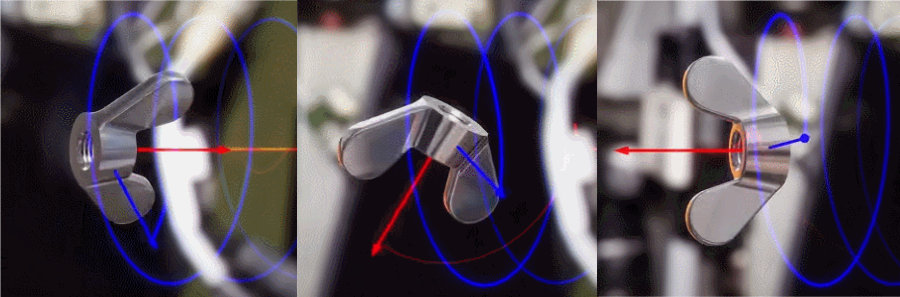
\includegraphics[width=0.9\textwidth]{dzhani.jpg}
\end{center}
   \caption{잔니베코프 효과  \cite{28}}
\label{fig:10}
\end{figure*}

\subsection{31번째 경도를 따라 발생한 104도 회전에 대한 물리적 증거}


이 회전 방향을 뒷받침하는 물리적 증거에는 고지자기, 판구조론, 사막, 생물 다양성, 고대 해류, 빙하 표석 데이터를 포함합니다.

그림 \ref{fig:7}에 보이는, 아이슬란드 분지와 라샹프 지자기 회유의 지자기 극 경로를 보존하고 있는 고지자기 데이터 연구 \cite{35}는 극이 대략적으로 동쪽 ECDO 회전축 (0 N, 121 E)주변을 회전하는 것을 보여준다. 이 자료는 극 회유 발생 동안 형성된 암석내 특정 자기 광물에 기록되어 있으며, 그 당시 지구 자기장의 방향과 강도에 대한 정보를 보존하고 있다.

지각이 부서지고 변형된 지각의 전단(단층) 평면에 대한 연구(그림 \ref{fig:8})에서도  동일한 패턴이 보여진다. 네덜란드의 지구 물리학자인 펠릭스 마인즈는 그의 논문에서 \cite{36} 이 패턴의 가장 가능성 있는 이유는 지구 회전축의 변화라고 설명하고 있다.

세계 주요 사막과 생물 다양성 핫스팟의 위치 또한 이 패턴과 일치한다. 사막들은 퇴적물과 함께 심하게 침수될 것으로 예상되는 위치에 존재하며, 반면 생물 다양성 핫스팟은 대양의 이동으로 심하게 타격받지 않을 지역에 존재합니다 \cite{28}. 이러한 배치는 그림 \ref{fig:9}에 나타나 있다.

그와 같은 예측된 ECDO 회전 경로에 대한 일치성은  미국 서부 사암층에 보존된 고대 해류 최적물과 빙하 표석에서도 존재한다. 표석은 추측컨데 빙하에 의해 집어 올려져 다른 암석 유형의 기반암에 퇴적된 바위로,  영국에서 이러한 표석은  ECDO 회전과 일치하는 예상 흐름 경로를 따른다 \cite{67,68}

\begin{figure*}[b]
\begin{center}
\includegraphics[width=1\textwidth]{layers.jpg}
\end{center}
   \caption{ECDO 뒤집힘을 초래하는 지구 내부 과정 \cite{129}}
\label{fig:11}
\end{figure*}

\begin{figure}[t]
\begin{center}
   \includegraphics[width=1\linewidth]{llvp.jpg}
\end{center}
   \caption{남아프리카 아래의 LLVP 세부 묘사 \cite{28}}
\label{fig:12}
\label{fig:onecol}
\end{figure}

\section{ECDO 뒤집힘을 설명하는 인과 물리학}

지구 회전축의 급격한 변화의 원리는 회전 물체와 관련한 물리학에 있다. 이의 전형적인 예는  그림 \ref{fig:10}에 있는 러시아 우주비행사 블라디미르 잔니베코프가 발견한 잔니베코프 효과 \cite{37}이다. 회전하는 물체가 관성에 따른 세 개의 주축들 중 하나위에서 정확하게 회전하지 않을 때, 물체는 고정된 회전축을 유지하지 않는다. 만약 그 물체가  두 번째 주관축 근처에서 회전할 경우, 그것은 회전에 있어 갑작스러운 변화를 겪게 된다. 이것이 우리가 지구의 급격한 뒤집힘 동안 일어날 것으로 믿는 것과 정확히 일치하지는 않지만, 중요한 점은 외부 힘이 없는 경우, 오직 회전 물리학만이 지구의 회전축의 급격한 변화를 설명할 수 있다는 것이다.

정확히 말하자면, 지구는 단순하고 균일한 잔니베코프 효과를 경험하지 않는 다는 것은 거의 확실하다. 만약 이와 같다면, 우리는 시간이 지남에 따라 지구 회전축의 점진적인 변화를 감지할 수 있을 것이다. 오히려, 우리는 지구가 주기적이고 갑작스러운 물리적 구조의 일탈과 이로인한 "외부 회전"(지각/맨틀)과 "내부 회전체"(핵)의 분리를 초래한다고 믿는다. 외부로부터 물리적 힘이 가해지지 않을 때, 각운동량 보존 법칙은 지구가 갑작스럽게 회전축을 변경할 수 없음을 보여주며, 따라서 외부와 내부 회전체의 분리, 즉 핵과 맨틀/지각의 분리는 갑작스럽고 급작스러운 지구 뒤집힘을 일으킬 수 있는 몇 가지 원인 중 하나이다.

지구 내부의 분리를 유도하는 특정 과정은 지구의 핵을 구성하고 있는 철의 구조적 변화라고 믿어진다(그림 \ref{fig:11}). 내핵은 육각형의 밀집된 철(Fe)로 이루어져 있다 \cite{141}. 이 hcp-Fe가 액상 금속의  상태로 변환될 때,  운동 에너지를 방출하면서서 외핵으로 떨어져 나간다. 이러한 고체에서 액체로의 상의 변화는 핵의 자기적 투과성을 감소시켜 지자기를 약화시키고, 열을 방출하여 맨틀에 LLVP(대규모 저속 전단 지역)구조를 생성하며(그림 \ref{fig:12}) \cite{38}, 심해를 통해 지구 표면을 가열합니다. 이 두 가지 경향은 최근 수세기에 걸쳐 잘 문서화되어 있으며, 이 논문 후반부에서 다루고 있다.

지구 내부에서의 이와 같은 과정이 반대 방향으로 발생하면서, 뒤집힘이 발생한 후 비교적 짧은 시간 뒤에 원래의 지구의 현재 회전 상태로의 전환을 유도한다고 믿어진다.

\section{임박한 지구 뒤집힘에 대한 증거}

\begin{figure}[t]
\begin{center}
   \includegraphics[width=1\linewidth]{npw.jpg}
\end{center}
   \caption{1590년부터 2025년까지 지자기 북극의 위치, 5년 단위로 묘사됨 \cite{142}.}
\label{fig:13}
\label{fig:onecol}
\end{figure}

\begin{figure*}[t]
\begin{center}
\includegraphics[width=0.9\textwidth]{saa.jpg}
\end{center}
   \caption{gufm1 및 IGRF-14 모델을 사용하여 계산된 1590년부터 2025년까지 약화된 지자기장 \cite{125,126}.}
\label{fig:14}
\end{figure*}

\begin{figure}[t]
\begin{center}
   \includegraphics[width=1\linewidth]{ocean-highlight.jpg}
\end{center}
   \caption{빨간색으로 표시되어 있는 1991년부터 2010년까지 2,000미터 이상의 깊이에서 심해 온난화 속도 \cite{132}.}
\label{fig:15}
\label{fig:onecol}
\end{figure}

우리는 또 다른 지구 뒤집힘의 문턱에 와 있다고 강력하게 믿는 이유가 있다. 수 천년 동안 대재앙이 발생하지 않았으며, 이 수천년의 기간은 역사적 기록과 데이터를 바탕으로 이러한 사건들이 발생하는 빈도와 대략적으로 일치한다. 임박한 뒤집힘을 뒷받침하는 가장 강력한 데이터는 최근 지구의 지자기장이 약 2000년 동안 약화되어 왔음을 보여주는 지자기의 데이터에서 나온다. 이러한 지자기의 약화느는 최근 몇 십 년 동안 가속화되고 있고, 경종을 울릴 만한 속도에 도달했다.

그림 \ref{fig:14}에 묘사된 것은 1590년과 2025년의 지구의 지자기장이다 \cite{125,126}. 그림에서 보이는 것처럼, 지자기장이 상당히 약화되었다.

약화되는 지자기장의 또 다른 지표는 지자기 북극의 위치이다 (그림 \ref{fig:13}). 역사적으로 지자기 북극은 캐나다 북극 지역에 위치해 있었다. 그러나 그 위치가 지난 몇 세기 동안 천천히 이동하고 있으며, 몇 십년 전부터 상당히 가속화되었다. 현재는 매년 55킬로미터의 속도로 러시아를 향해 빠르게 이동하고 있다 \cite{124}.



지구의 자기장은 내부 다이너모, 즉 지구 외핵에서 회전으로 인해 움직이는 마그마 흐름의 원형 기둥에 의해 생성되는 것으로 믿어집니다 \cite{123}. 약화되는 지자기장은 지구 깊숙한 곳에서 일어나는 변화의 증상이다. ECDO 이론에 따르면, 이러한 혼란은 열을 방출하고 결국 맨틀과 핵의 분리를 일으켜 지구 뒤집힘을 초래한다 \cite{1}.

지구 내부 발열성 과정의 존재를 입증하는 상당한 데이터가 있다. 지구 온난화는 대륙 및 대양 표면 온도의 상승 \cite{127,128}, 지구 열기둥과 함께  움직이는 대기 중 CO2 수치의 상승 \cite{129,130}, 전 세계 해빙 면적의 감소 \cite{131}에서 입증되었다. 데이터는 CO2 수치 및 온도 상승이 "인위적" 기후 변화의 원인이 아니라, 오히려 발열성 핵의 하류 효과임을 시사합니다 \cite{129}.

가장 중요하게는, 심해(깊이 $>$2000 미터)의 온난화 속도에 대한 연구는 깊은 바다가 온난화되고 있을 뿐만 아니라, 심해저층(4000 - 6000 미터)에서 가장 빠른 온난화 속도를 보인다는 것이다. 이러한 심해 온난화는 4000미터 아래에 그 산술평균의 중심점을 가지고 있으며\cite{132,129}, 이는 대기에 의해  해양이 가열되고 있다면 불가능할 것이다. 이러한 자료는 최근의  기후 및 지자기 변동이 지구 내부 깊은 곳에서 일어나고 있는 일련의 과정에 의해 촉발되고 있음을 강력하게 뒷받침한다. 그림 \ref{fig:15}는 1991년부터 2010년까지 전 세계 심해의 온난화 속도를 묘사한다 \cite{132}.

\section{임박한 지구 뒤집힘의 모델링}

\begin{figure}[b]
\begin{center}
   \includegraphics[width=1\linewidth]{saa-crop.jpeg}
\end{center}
   \caption{남대서양 이상 현상을 기반으로 계산된 특이한 결정적 전환점, 2059년 3월 13일 \cite{125,126}.}
\label{fig:16}
\label{fig:onecol}
\end{figure}

지구의 다음 뒤집힘 시기를 예측하는 것은 매우 복잡한 작업이다. 현재 이러한 작업에 적합한 최상의 모델은 남대서양 이상 현상 (SAA)이라는 지구자기장이다. 남대서양 상공에 있는 지자기장 영역은 1590년 지구 지자기장 측정시 최저치였던 32,000 나노테슬라 \cite{135}이하의 자기장 영역을 말한다. 남대서양 이상 지역의 표면적은 1590년 지구 표면의 1%에서 2025년에는 1%로 증가했다\cite{136}.


지구가 언제 뒤집힐지를 추정하기 위해, 나는 SAA 표면적 데이터를 복잡한 시스템이 급격한 변화에 이르는 임계 전환에 접근하는 것을 모델링하는 멱법칙 전환점 방정식에 대입했다. 계산 결과, 나온 전환점 예측 날짜는 2059년 3월 13일이다(그림 \ref{fig:16}). 이 예측은 전환시기에 가까워질수록 점점 더 정확해질 것이다\cite{136}.

또한 회전축의 일탈, 기상 이변, 그리고 지진 및 화산 데이터등의 다른 지표들은 우리가 다음 지구 뒤집힘이 언제 발생할 것인가에 대해 더 나은 예측을 할 수 있도록 도움을 줄 수 있다.

\section{ECDO의 역사적 연대표}

과거에 발생한  ECDO 사건의 정확한 타임라인을 설정하는 것은 어렵지만, 홀로세 즉 현세 동안 최소 2번의 ECDO 사건이 있었던 것으로 보인다. 헤로도토스가 이집트 사제의 이야기에서 언급한 것을 주목하자. \textit{"첫 번째 왕부터 마지막으로 통치했던 헤파이스토스 사제까지, 사람의 세대가 341번 바뀌었다....이 시간 동안 그들은 해가 원래 떠오르던 곳에서 네 번이나 움직였고, 지금 해가 지는 곳에서 두 번 떠올랐으며, 지금 해가 뜨는 곳에서 두 번 졌다"} \cite{32}. 기원전 5세기에 살았던 플라톤은 9000년 전 단 하루 동안 아틀란티스를 물에 잠기게 했던 홍수 뒤에,\textit{"그 이후로 많은 대홍수가 있었고, 산에 살아남은 후세는 글쓰기를 몰랐으며, 그리고  여러 세대에 걸쳐 생존 수단을 얻는 데 전념했다"} \cite{112}라고 하며, 이는 약 기원전 9700년 경 소멸된 소빙하기 이후 두 번 이상의 뒤집힘이 있었음을 시사한다. 이 논문과 내 연구에서 다룬 물리적 증거 \cite{2}는 플라톤의 말을 뒷받침하는 풍부한 증거를 제공한다.

가장 최근 ECDO 뒤집힘 시기의 후보는  많은 대재앙적 홍수 기록(Gun-Yu \cite{113,114,115}이 있는 기원전 2300년에서 1600년 사이로, 오기게스 \cite{116,117}, 페루 \cite{118,119}, 출애굽 \cite{120}), 문명 파괴와 유기(모헨조다로 \cite{121}, 미노아 크레타\cite{100,101}) 및 물리적 이상현상 (본드 이벤트 \cite{122}, 4.2킬로년 이벤트 \cite{90})가 그 시기로 기록되어 있다. 이후 주요한 대재앙적 사건을 시사하는 충분한 증거의 수렴은 없습니다.

\section{결론}
작전 NANOOK는 2차 세계대전 후 미국이 북극과 북부 소련 해안을 탐색하기 위한 냉전 시기의 정찰 활동이었다 \cite{137}. 그들은 조사 활동 중, 자극이 이전 탐험시 발견된 자료에 근거해 예상되었던 위치보다 북쪽으로 125에서 200마일 떨어져 있다는 것을 발견했다. 따라서, \textit{"정부 과학자들 사이에서는 자기극과  지리학적 극이 일치할 때 무엇이 일어날지에 대한 질문이 생겼다. 이에 대한 해답을 찾기 위해, Dr. Paul A. Siple의 프로젝트 지휘 하에, Rand Corporation은 동심 구형의 지구 모델들을 사용하여  실험실 연구를 진행하기 위해 계약을 맺었다. - 전자기적으로 충전된 지구의 용융 철로 구성된 핵을 나타내며, 그 축이 자기극이라 정의된 안쪽 구형 ; 그리고 "지리적" 극을 축으로 회전하는 지구의 지각을 나타내는 바깥쪽 구형. 반복된 실험을 통해 "자기" 극이 "지리적" 극에 접근함에 따라, 어느 시점에서 구심력에 의해  "자기" 극이 "지리적" 극으로 끌려가는 속도가 급가속하며 일치하기 위해 돌진할 수 있다. ;그러나 두 극이 일치하는 대신, "자기" 극이 "지리적" 극 주위를 급격히 튕기듯 돌며 , 원심력에 의해 분리되면서 적도를 향해 회전하면서 두 축이 약 89도의 각도로 이탈하는 위치에 놓이게 된다는 것이 발견되었다. 극 "튀어오름" 후부터, 두 축이 오랜 시간에 걸쳐 점차 재수렴하기 시작할 것이다."} \cite{138,139}.

이어서, \textit{"1948년 초 화이트 소령이 펜타곤에서 참석한 과학 회의들 중 하나에서, 과학자들은 대중에게 당면한 극 역전  현상에 대해 알리는 것의 득실에 대해 논의하였다. 과학자들 중 누구도 대중에게 이 정보를 숨기는 것에 동의하지 않았다; 그러나 반면에,어떻게 공개할 것인지에 대해 합의하지도 못했다. 이 현상에 대한 정보는 그 자체로 사회의 도덕적 결속을 파괴할 수 있다는 의견도 있었다. 그러나 1950년대 초에, 튀어오름 현상에 대한 정보가 신문의 칼럼과 잡지 기사로 공개되었을 때 , 놀랍게도 어안이 벙벙하고 편협하거나 의심많은 대중들은 아무 반응도 없었고, 앞선 과학자들의 두려움은 근거없는 것이 되었다."} \cite{138,139}.

왜 우리는 이것에 주의를 기울이지 않는가? 지구가 과거에 뒤집혔다고 믿을만한  충분한 이유들이 있다. 제 2부 논문과 함께 이 논문은 전 세계의 홍수 이야기들, 대륙을 덮고 있는 소금 및 해양 화석, 고대 지하 대피소들, 동물 유해들 및 파괴적인 지질학적 풍경들과 같이 지구 뒤집힘을 시사하는 수많은 증거들을 밀도있게 요약하여 다루고 있다. 인류는 수십만 년 동안 존재해온 것으로 추정되지만, 현대사는 몇천 년 전까지밖에 거슬러 올라가지 않는다. 어쩌면 종종 지구가 뒤집히면서 대륙이 깨끗이 청소되고, 우리는 고대 역사의 기록을 몇 가지의 파괴적인 이야기로 줄이면서 석기 시대 즉, 원점으로 돌아가야 하는 것이 아닌가? 그렇다면, 이것이 다시 발생하지 않도록 막는 것이 인류의 가장 중요한 임무 중 하나일 수 있다.

마지막으로, 나는 플라톤이 아테네 정치가 솔론과  이집트 사제들 간의 대화를 기록한  티마이오스에 자세히 기록한  다음의 이야기를 남기고자 한다. \cite{140}: \textit{"그리고 한 번은 [솔론]이 그들을 고대 역사에 대한 토론에 끌어드렸을 때, 그는 가장 오래된 우리의 전통들과 첫번째 사람으로 언급되는 포로네우스와 니오베에 관하여 그들에게 이야기하고자 했다.; 또한 솔론은  홍수 후의 데우칼리온과 피라의 전설과 그들이 어떻게 생존했는지에 대해 이야기 했다. 또한 솔론은 언급된 사건들이 차지했던 년도의 횟두들을 계산함으로써, 시간의 주기들을 계산해보고자 했다. 그 때  나이 든 사제 중 한 명이 말했다, "오 솔론, 솔론, 당신들 그리스 인은 항상 아이들같다: 고대 그리스란 것은  존재하지 않는다." 이 말을 듣고 그는 물었다, "그 말은 무슨 뜻인가?" 그러자 사제가 답했다, "당신들의 영혼은 젊습니다. 모두가 그러하죠. 왜냐하면 여러분은 고색창연한 과학문명은 커녕 오래된 그리고 예로부터 물려받은 신념도 전혀 없습니다. 그리고 이것이 그 원인입니다: 인류에 많은 다양한 파멸이 있었고, 앞으로도 있을 것입니다, 가장 큰 파멸은 불과 물에 의한 것이며, 더 작은 파괴들은 무수한 다른 것들에 의한 것입니다. 실제로  우리 나라뿐만 아니니라 당신 나라에서 회자되는 이야기, 아주 오래 전 헬리오스의 아들 파에톤이 어떻게 아버지의 전차에 멍에를 메었고, 또 아버지가 전차를 몰았던 경로를 따라 운전을 하지 못했기 때문에 지상의 것들을 태우고 그 자신은 벼락에 맞아 죽었는지에 대한 이야기기는 말 그대로 전설의 형식을 가지고 있습니다. 그러나 그 실상은 하늘에서 지구를 중심으로 도는 물체의 이동의 출현과 오랜 간격을 두고 재발하는 격렬한 불에 의한 파괴에 있습니다. 이런 시기에, 산과 높고 건조한 곳에 사는 사람들이 강이나 바다 근처에 사는 사람들보다 더 많이 파괴로 고통받고; 우리 같은 경우 달리말해 우리의 구원자인라 할 수 있는 나일 강은 이런 시기에 우리를 재난에서 구원해 줍니다. 반면, 신들이 홍수로 지구를 정화할 때, 산에 있는 모든 목동과 양치기들은 구원을 받지만, 당신 나라의 도시인들은 해류에 의해  바다로 쓸려갑니다; 하지만 우리 나라는 그 시기에도 물이 위에서 아래로 우리 밭에 쏟아지지 않으며, 오히려 자연적으로 아래에서 샘솟곤 합니다. 그래서 여기서 보존된 것이 가장 오래되었다고 여겨집니다; 예방해야할 과도한 더위나 추위가 없는 모든 곳에는 숫자상으로 다소의 차이가 있지만, 늘 인류의 군락이 있었습니다. 그리고 고귀하거나 위대하거나 주목할 만한 사건이 발생한다면, 그것이 당신의 나라나 우리나라 또는 기록을 통해 아는 다른 어떤 곳에서든, 예로부터 그런 모든 사건들은 여기 우리 사원들에 기록되고 보존되었습니다; 반면에 당신 나라 사람들과 다른 이들은 문명화된 국가들이 필요로 하는 언어와 모든 인문과학을 다시 갖추지만, 전염병과도 같이, 보통 수 년 뒤 다시  하늘에서의 홍수가 당신 나라의 사람들에게 쏟아지면, 여러분 중 누구도 문자 되지 않은 자 외에는 살아남지 못합니다, 그래서 당신들은 다시 젊어지게 되고, 우리 나라와 당신의 나라에서 이미 있었던 모든 일들에 대한 지식을 지니고 있지 못합니다. 솔론 확실히 당신이 방금 언급한  당신 나라의 사람들에 대한 계보는 어린아이의 이야기와 다를 바가 없습니다; 왜냐하면, 첫째로, 이전에 많은 대홍수가 있었지만, 당신은 단 하나의 홍수만을 기억합니다.; 두 번째로, 당신은 인류 중 가장 고귀하고 완벽한 인종이 당신들이 지금 살고 있는 땅에서 태어났고, 몇몇 남겨진 자손들로부터 당신 자신은 물론이고 현재 존재하는 당신의 도시 전체가 태어났지만, 이 사실을 모릅니다. 왜냐하면 여러 세대에 걸쳐 생존자들이 그들 자신을 글로써 표현할 능력을 갖지 못하고 사라졌기 때문입니다. 솔론, 진정 오래 전 물에 의한 가장 큰 파멸이 있기 전에는, 지금의 아테네 국가가 전쟁에서 가장 용감했고, 또 다른 모든 면에서도 매우 잘 조직되어 있었습니다. 그 나라가 우리가  들었던 하늘 아래의 모든 국가 중 가장 훌륭한 예술 작품과 고귀한 통치 체제를 갖고 있었다고 합니다."}. 

물론 이들 사제들은  솔론에게 아틀란티스의 고대 문명에 대해서도 이야기했다: \textit{"우리가 여기서 이야기한 것들은 분명 좁은 문을 가진 천국입니다. 반면에 저쪽은 진정한 대양이며, 그것을 둘러싸고 있는 땅은 가장 완전하고 진정한 의미에서의  대륙이라고 부를 수 있습니다. 이제 이 아틀란티스 섬에는 위대하고도 경이로운  권력을 가진 왕들의 연합이 존재하였으며, 그 힘은 아틀란티스 섬 전체뿐만 아니라  다른 여러 섬들 그리고 대륙의 일부에까지 영향력을 미쳤습니다.; 더 나아가 그들이 지배했던 해협내의 이집트까지  이르는 리비아의 땅과 티레니아에 이르는 유럽을 지배했습니다. 그리하여 한 때 이 연합군이 모두 모여  당신의 나라와 우리 나라, 그리고 해협 내의 모든 영토를 한 번의 맹공격으로  노예로 만들려고 시도했습니다.솔론, 그때 당신의 나라의 남자들은 눈에 띄는 용멩함을 보였으며, 전 세계 사람들이 보기에도 그러했을 것입니다. 용감함과 모든 전쟁 기술에서 모두 출중했고, 부분적으로  그리스인의 지도자로서 행동하고, 일부는 다른 모든 이들에 의해 버려졌을 때 홀로 섰기 때문에, 가장 치명적인 위기를 겪은 후에 침입자를 물리치고 승전의 트로피를 들어올렸습니다.; 이에 따라 아직 노예가 되지 않은 사람들을 노예제도도에서 구하고, 헤라클레스 경계 내에 거주하는 우리 모두를 자유롭게 해방했습니다. 그러나 후에 엄청난 지진과 홍수가 발생했으며, 땅이 당신의 전사들을 삼키고 아틀란티스 섬이  바다에 삼켜져 사라지는 비통한 낮과 밤이 그들에게 들이닥쳤습니다."}

\section{감사의 글}

윤리적 회의론이자 ECDO 논문의 원저자인 Ethical Skeptic에게 통찰력 있고 혁신적인 논문을 완성하고 세상과 공유해주신 것에 대해 감사드립니다.. 그의 3부작 논문\cite{1}은 발열성 핵-맨틀 분리 잔니베코프 진동(ECDO) 이론의 새로운 획을 긋는 작업이며, 이 주제에 대해, 내가 여기에서 간단히 다룬 것보다 훨씬 더 많은 정보를 담고 있다.

표 1에서 대재앙 자료와 기록을 집계하고 처리한 Ankit에게 감사합니다.

그리고 당연히, 이 작업을 가능하게 했고 인류에 광명을 가져다 준 연구와 조사를 했던 모든 위대한 이들에게 감사드립니다.

\clearpage
\twocolumn

\section{추가 이미지}

\begin{figure}[H]
\begin{center}
   \includegraphics[width=1\linewidth]{wave.jpg}
\end{center}
   \caption{카프레 피라미드에 있는 포물선형 하부 침식에 대한 자세한 관찰 \cite{27}.}
\label{fig:17}
\label{fig:onecol}
\end{figure}

\begin{figure}[H]
\begin{center}
   \includegraphics[width=1\linewidth]{star-stone.jpg}
\end{center}
   \caption{쿠푸 피라미드의 한 통로에 새겨진 별 지도 \cite{28}.}
\label{fig:18}
\label{fig:onecol}
\end{figure}

\begin{figure*}[t]
\begin{center} 
\includegraphics[width=1\textwidth]{deepsea.jpg}
\end{center}
   \caption{대기의 작용에 의한 정상적인 해양 가열 곡선과 비교한 심해층 및 심해대의 해양 이상 가열  현상의 시각화.  NOAA의 전체 이상 가열 현상 자료는, \cite{147}, Desbruyeres의 심해 및 심해 가열 분포 연구자료 및 \cite{132},  Ethical Skeptic의 데이터 처리 및 시각화 자료를 인용했다.   \cite{129}.}
\label{fig:19}
\end{figure*}

\begin{figure*}[t]
\begin{center}
\includegraphics[width=1\textwidth]{sealevel.jpeg}
\end{center}
   \caption{해류 속도의 증가와 함께 75년에 걸쳐 63개 지점에서  20\%가 넘는 변동성을 보여주는 해수면. 해수면 변동성의 급증은 해양 열 파동와 동시에 발생하며, 이는 이들 모두  지구의 심해  래로부터의 가열로 인해 발생할 수 있음을 나타낸다. \cite{2,129}.}
\label{fig:20}
\end{figure*}

\begin{figure*}[t]
\begin{center}
\includegraphics[width=1\textwidth]{co2.jpg}
\end{center}
   \caption{ 지난 45년 동안 꾸준히 증가한 대기 중 CO2 농도. 이는 해양 온도의 상승으로 인해 발생했을 가능성이 높음. 출처: NOAA \cite{148,129}.}
\label{fig:21}
\end{figure*}

\begin{figure*}[t]
\begin{center}
\includegraphics[width=1\textwidth]{ice.jpg}
\end{center}
   \caption{지난 45년 동안 지구의 온난화로 인해 줄어들고 있는 지구 해빙 면적. 출처: ADS \cite{149}.}
\label{fig:22}
\end{figure*}

\clearpage
\twocolumn

{\small
\bibliographystyle{ieee}
\bibliography{egbib}
}

\end{document}